\documentclass[12pt]{exam}

\usepackage[utf8]{inputenc}  % For UTF8 source encoding.
\usepackage{amsmath}  % For displaying math equations.
\usepackage{amsfonts} % For mathematical fonts (like \mathbb{E}!).
\usepackage{upgreek}  % For upright Greek letters, such as \upvarphi.
\usepackage{wasysym}  % For additional glyphs (like \smiley!).
\usepackage{mathrsfs} % For script text (hash families and universes).
\usepackage{enumitem}
\usepackage{graphicx}
% For document margins.
\usepackage[left=.8in, right=.8in, top=1in, bottom=1in]{geometry}
\usepackage{lastpage} % For a reference to the number of pages.
\usepackage[table,xcdraw]{xcolor}
\usepackage{pdfpages}
\usepackage{verbatim}
\usepackage{afterpage}
\usepackage{listings}
\usepackage{color} %red, green, blue, yellow, cyan, magenta, black, white
\definecolor{mygreen}{RGB}{28,172,0} % color values Red, Green, Blue
\definecolor{mylilas}{RGB}{170,55,241}

\newcommand*{\authorname}{Luis A. Perez}

\newcommand*{\duedate}{Wednesday, August 14th}
\newcommand*{\duetime}{11:59 pm}

% Fancy headers and footers
\headrule
\firstpageheader{EE 263\\Summer 2019}{Homework 7 \\ }{Due: \duedate\\at \duetime}
\runningheader{EE 263}{Homework 7}{\authorname}
\footer{}{\footnotesize{Page \thepage\ of \pageref{LastPage}}}{}

% Exam questions.
\newcommand{\Q}[1]{\question{\large{\textbf{#1}}}}
\qformat{}  % Remove formatting from exam questions.

% Useful macro commands.
\newcommand*{\bigtheta}[1]{\Theta\left( #1 \right)}
\newcommand*{\bigo}[1]{O \left( #1 \right)}
\newcommand*{\bigomega}[1]{\Omega \left( #1 \right)}
\newcommand*{\prob}[1]{\text{Pr} \left[ #1 \right]}
\newcommand*{\ex}[1]{\text{E} \left[ #1 \right]}
\newcommand*{\var}[1]{\text{Var} \left[ #1 \right]}

\newcommand*{\norm}[1]{\left\lVert #1 \right\rVert}
\newcommand*{\HH}{\mathscr{H}}   % Family of hash functions.
\newcommand*{\UU}{\mathscr{U}}   % Universe.
\newcommand*{\eps}{\varepsilon}  % Epsilon.


% Custom formatting for problem parts.
\renewcommand{\thepartno}{\roman{partno}}
\renewcommand{\partlabel}{\thepartno.}

% Framed answers.
\newcommand{\answerbox}[1]{
\begin{framed}
\hspace{\fill}
\vspace{#1}
\end{framed}}

\printanswers

\setlength\answerlinelength{2in} \setlength\answerskip{0.3in}

\begin{document}
\title{EE 263 Homework 7}
\author{\authorname}
\date{}
\maketitle
\thispagestyle{headandfoot}
\setcounter{MaxMatrixCols}{15}

\lstset{language=Matlab,%
    %basicstyle=\color{red},
    breaklines=true,%
    morekeywords={matlab2tikz},
    keywordstyle=\color{blue},%
    morekeywords=[2]{1}, keywordstyle=[2]{\color{black}},
    identifierstyle=\color{black},%
    stringstyle=\color{mylilas},
    commentstyle=\color{mygreen},%
    showstringspaces=false,%without this there will be a symbol in the places where there is a space
    numbers=left,%
    numberstyle={\tiny \color{black}},% size of the numbers
    numbersep=9pt, % this defines how far the numbers are from the text
    emph=[1]{for,end,break},emphstyle=[1]\color{red}, %some words to emphasise
    %emph=[2]{word1,word2}, emphstyle=[2]{style},    
}

\begin{questions}
%%%%%%%%%%%%%%%%%%%%%%%%%%%%%%%%%%%
  \Q{Bow Tie Launch}

  \begin{solution}
    \begin{enumerate}[label=(\alph*)]
      \item Given the restrictions imposed by the problem, we begin by tackling it in pieces. First, note that we can write $x(t)$ in the following form:
      \begin{align*}
        x(t) &= \begin{bmatrix} A^{t-1}B & A^{t-2}B & \cdots & AB & B \end{bmatrix}u_{\text{seq}} \\  &+ (A^{t-1} + A^{t-2} + \cdots + A + I)B_g \\
      \implies
        x(t) - (A^{t-1} + A^{t-2} + \cdots + A + I)B_g &= \begin{bmatrix} A^{t-1}B & A^{t-2}B & \cdots & AB & B \end{bmatrix}u_{\text{seq}} \\
        \implies \begin{bmatrix} e_1 \\ e_3 \end{bmatrix} [x(t) - (A^{t-1} + A^{t-2} + \cdots + A + I)B_g] &=  \begin{bmatrix} e_1 \\ e_3 \end{bmatrix}\begin{bmatrix} A^{t-1}B & A^{t-2}B & \cdots & AB & B \end{bmatrix}u_{\text{seq}}  \\
        \implies p(t) - \begin{bmatrix} e_1 \\ e_3 \end{bmatrix}(A^{t-1} + A^{t-2} + \cdots + A + I)B_g &= \begin{bmatrix} e_1 \\ e_3 \end{bmatrix}\begin{bmatrix} A^{t-1}B & A^{t-2}B & \cdots & AB & B \end{bmatrix}u_{\text{seq}}
      \end{align*}
      which is very nearly in the form we're trying to find, given by:
      \[
        \hat{A}u_{\text{seq}} = \hat{y}
      \]
      In fact, we can let:
      \[
        \hat{y}_t = p(t) - \begin{bmatrix} e_1 \\ e_3 \end{bmatrix}(A^{t-1} + A^{t-2} + \cdots + A + I)B_g \in \mathbb{R}^2
      \]
      and then we can define:
      \[
        \hat{y} = 
          \begin{bmatrix}
            y_{10} \\
            y_{20} \\
            \vdots  \\
            y_{60} \\
            y_{61} \\
            \vdots \\
            y_{65}
          \end{bmatrix} \in \mathbb{R}^{22}
      \]
      With the above defined, we can similarly create our matrix $\hat{A}$. First, let us defined:
      \[
        \hat{A}_t = \begin{bmatrix} e_1 \\ e_3 \end{bmatrix}\begin{bmatrix} A^{t-1}B & A^{t-2}B & \cdots & AB & B & 0 & \cdots & 0 \end{bmatrix} \in \mathbb{R}^{2 \times 130} \tag{Where the front is padded by $0$s}
      \]
      Then we define our matrix $\hat{A}$ simply as:
      \[
        \hat{A} = 
          \begin{bmatrix}
            \hat{A}_{10} \\
            \hat{A}_{20} \\
            \vdots \\
            \hat{A}_{60} \\
            \hat{A}_{61} \\
            \vdots \\
            \hat{A}_{65} \\
          \end{bmatrix} \in \mathbb{R}^{22 \times 130}
      \]
      Then note that we immediately have the system as desired:
      \[
        \hat{y} = \hat{A}u_{\text{seq}}
      \]
      Solving for the minimum norm solutin, we have:
      \[
        u_{ln} = \hat{A}^T(\hat{A}\hat{A}^T)^{-1}\hat{y}
      \]
      A plot of the applied forces can be seen in Figure \ref{fig:least_norm_forces_drone}, and a plot of the calculated drone trajectory and waypoints in Figure \ref{fig:drone_trajectory}.


      \item

        This is just a weighed sum objective problem. The weighed sum objective can be rewritten as:
        \[
          J_1 + \mu J_2 = \left|\left|
          \begin{bmatrix}
            \hat{A} \\ \sqrt{\mu}I 
          \end{bmatrix}u_{\text{seq}} - \begin{bmatrix} \hat{y} \\ 0  \end{bmatrix} \right|\right|_2^2
        \]
        This should be immediately obvious, but for the wary, we show the argument below. Basically, expanding out we have:
        \begin{align*}
          J_1 + \mu J_2 &= \sum_{i=1}^{11} ||q(t_i) - p_i ||^2 + \mu \sum_{t=0}^{64}||u(t)||^2 \\
          &= \sum_{i=1}^{11} ||q(t_i) - X_{t_i} + X_{t_i} - p_i ||^2 + \mu \sum_{t=0}^{64}||u(t)||^2 \tag{$X_{t_i} = \begin{bmatrix} e_1 \\ e_3 \end{bmatrix}(A^{t_i-1} + A^{t_i-2} + \cdots + A + I)B_g$} \\
          &=\sum_{i=1}^{11} ||\hat{A}_{t_i}u(t_i) - \hat{y}_i ||^2 + \mu \sum_{t=0}^{64}||u(t)||^2 
        \end{align*}
        From the above, we can see how we can rewrite as described. As such, we have that the solutions are given directly by:
        \[
          u^* = \begin{bmatrix}
            \hat{A} \\ \sqrt{\mu}I 
          \end{bmatrix}^{\dagger}\begin{bmatrix} \hat{y} \\ 0 \end{bmatrix}
        \]
        where we note that $\begin{bmatrix} \end{bmatrix} \in \mathbb{R}^{87 \times 130}$, so it is fat and full-rank. As such we know exactly how to compute the solution.
        As such, we compute the above and vary the values of $\mu$ from $1 to 10^7$. The resulting trade-off curve is shown in Figure TODO (incomplete).

      \item We plot the five trajectories. See the attached figures.
      \item We find the matrices $F$ and $G$ so that we can rewrite the cost functions. We can immediately see that the matrix 
      \begin{align*}
        J_3 &= \sum_{t=0}^{65} ||q(t)||^2 \\
        &= \sum_{t=0}^{65} || A_tu_{\text{seq}} + \begin{bmatrix} e_1 \\ e_3 \end{bmatrix} (A^{t-1} + A^{t-2} + \cdots + A + I)B_g||^2 \tag{Results from (a)} \\
        &= || Wu_{\text{seq}} +  G||^2
      \end{align*}
      where we have $G$ given by:
      \[
        Z = \begin{bmatrix}
          0 \\
          \begin{bmatrix} e_1 \\ e_3 \end{bmatrix} B_g \\
          \begin{bmatrix} e_1 \\ e_3 \end{bmatrix} (A + I)B_g \\
          \vdots \\
          \begin{bmatrix} e_1 \\ e_3 \end{bmatrix} (A^{t-1} + A^{t-2} + \cdots + A + I)B_g
          \vdots \\
          \begin{bmatrix} e_1 \\ e_3 \end{bmatrix} (A^{64} + A^{63} + \cdots + A + I)B_g
        \end{bmatrix} \in \mathbb{R}^{130 \times 1}
      \]
      and
      \[
        W = 
          \begin{bmatrix}
            0 \\
            A_1 \\
            A_2 \\
            \vdots \\
            A_{65}
          \end{bmatrix} \in \mathbb{R}^{130 \times 130}
      \]
      With the above, we have the full objetive as:
      \[
        J_3 + \gamma J_2 = ||W u_{\text{seq}} + Z||^2 + \gamma||u_{\text{seq}}||^2
      \]
      We can do the same trick we did for the multi-objective function, and combine the above into one norm as follows:
      \[
        J_3 + \gamma J_2 = ||F u_{\text{seq}} + G ||^2 
      \]
      where we write:
      \[
        F = \begin{bmatrix}
          W \\
          \sqrt{\gamma}I
        \end{bmatrix}
      \]
      and 
      \[
        G = 
          \begin{bmatrix}
            Z \\
            0
          \end{bmatrix}
      \]
      so that it matches the output dimensions of $F$.

      \item
        We show that the optimal solution to a problem of the form
        \begin{align*}
          \text{minimize} && ||Fu + G||^2  \\
          \text{subject to} && \hat{A}u = \hat{y}
        \end{align*}
        is given by:
        \[
          u_{\text{opt}} = \Sigma^{-1}\hat{A}^T(\hat{A}\Sigma^{-1}\hat{A}^T)^{-1}(\hat{y} + \hat{A}\Sigma^{-1}F^TG) - \Sigma^{-1}F^TG
        \]
        We can do this using Lagrange multipliers. The Lagrangian for our problem is given by:
        \begin{align*}
          L(u, \lambda) &= (Fu + G)^T(Fu + G) + \lambda^T(\hat{A}u - \hat{y}) \\
          &= u^T\Sigma u + G^TG + u^TFG + GFu + \lambda^T(\hat{A}u - \hat{y})
        \end{align*}
        This gives the optimality conditions as:
        \begin{align*}
          \nabla_{u} L = 2u^T\Sigma + \textbf{1}^T FG + \textbf{1}^T GF + \lambda^TA = 0  \\
          \nabla_{\lambda} L = \hat{A}u - \hat{y} = 0 
        \end{align*}
        The first condition immediate gives:
        \[
          u = -\frac{1}{2}\Sigma^{-1}(\hat{A}^T\lambda + 2F^TG)
        \]
        We can then subtitute this solution into the second equation to give us:
        \begin{align*}
          -\frac{1}{2}\hat{A}(\Sigma^{-1}(\hat{A}^T\lambda + 2F^TG)) = \hat{y} \\
          \implies \lambda = -2(\hat{A}\Sigma^{-1}\hat{A}^T)^{-1}(\hat{y} + \hat{A}\Sigma^{-1}F^TG)
        \end{align*}
        and finally, subtituting $\lambda$ back into the first equations we have:
        \begin{align*}
          u_{\text{opt}} &= \Sigma^{-1}\hat{A}^T(\hat{A}\Sigma^{-1}\hat{A}^T)^{-1}(\hat{y} + \hat{A}\Sigma^{-1}F^TG) - \Sigma^{-1}F^TG
        \end{align*}
        just as we wanted.
      \item The plots for the values are shown in the attached code. We can see in the plots the clear tradeoff for $\gamma$. A low value of $\gamma$ causes the drone to try extremely hard to stay close to the origin. The case with. the $\gamma = 10$ seems to match the requirements the best.
      \item See attached code for attempt at plotting the trade-off curves.
    \end{enumerate}
  \end{solution}


  \begin{figure}[hpb!]
    \centering
    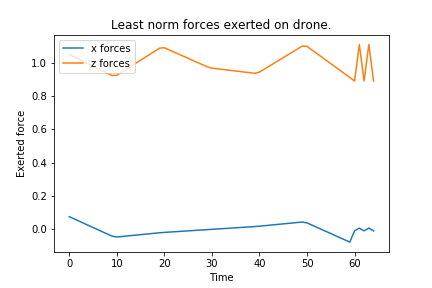
\includegraphics[scale=1.0]{least_norm_forces.png}
    \caption{Plot of least norm forces over time.}
    \label{fig:least_norm_forces_drone}
  \end{figure}

  \begin{figure}[hpb!]
    \centering
    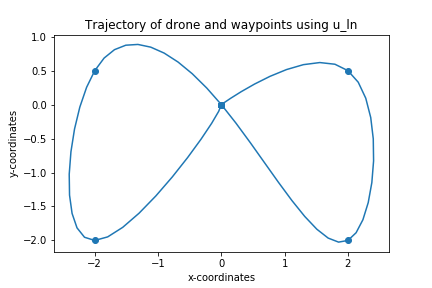
\includegraphics[scale=1.0]{drone_trajectory.png}
    \caption{Waypoint and drone trajectory}
    \label{fig:drone_trajectory}
  \end{figure}


  \newpage
  \Q{Attack position of Fighter Jets}

  \begin{solution}
    \begin{enumerate}[label=(\alph*)]
      \item Following the hint, we try to express each of the control schemas as a linear dynamical system. That is to say, we try to frame them in the form:
      \[
        \dot{x} = Ax
      \]
      where $x$ is our state vector. 
      \begin{itemize}
        \item \textit{Right looking control}:

          For this control schema, we begin by defining our state as follows:
          \[
            x =
              \begin{bmatrix}
                y_n \\ s_{n-1} \\ s_{n-2} \\ \vdots \\ s_1 \\ v_n \\ v_{n-1} \\ \vdots \\ v_1 \\ 1
              \end{bmatrix} \in \mathbb{R}^{2n + 1}
          \]
          This leads us to the matrix $A$ (in our case $n = 7$) defined as:
          \[
            A =
              \begin{bmatrix}
                0 & 0 & 0 & 0 & 0 & 0 & 0 & 1 & 0 & 0 & 0 & 0 & 0 & 0 & 0 \\
                0 & 0 & 0 & 0 & 0 & 0 & 0 & 1 &-1 & 0 & 0 & 0 & 0 & 0 & 0 \\
                0 & 0 & 0 & 0 & 0 & 0 & 0 & 0 & 1 &-1 & 0 & 0 & 0 & 0 & 0 \\
                0 & 0 & 0 & 0 & 0 & 0 & 0 & 0 & 0 & 1 &-1 & 0 & 0 & 0 & 0 \\
                0 & 0 & 0 & 0 & 0 & 0 & 0 & 0 & 0 & 0 & 1 &-1 & 0 & 0 & 0 \\
                0 & 0 & 0 & 0 & 0 & 0 & 0 & 0 & 0 & 0 & 0 & 1 &-1 & 0 & 0 \\
                0 & 0 & 0 & 0 & 0 & 0 & 0 & 0 & 0 & 0 & 0 & 0 & 1 &-1 & 0 \\
               -1 & 0 & 0 & 0 & 0 & 0 & 0 &-1 & 0 & 0 & 0 & 0 & 0 & 0 & 7 \\
                0 & 1 & 0 & 0 & 0 & 0 & 0 & 0 &-1 & 0 & 0 & 0 & 0 & 0 &-1 \\
                0 & 0 & 1 & 0 & 0 & 0 & 0 & 0 & 0 &-1 & 0 & 0 & 0 & 0 &-1 \\
                0 & 0 & 0 & 1 & 0 & 0 & 0 & 0 & 0 & 0 &-1 & 0 & 0 & 0 &-1 \\
                0 & 0 & 0 & 0 & 1 & 0 & 0 & 0 & 0 & 0 & 0 &-1 & 0 & 0 &-1 \\
                0 & 0 & 0 & 0 & 0 & 1 & 0 & 0 & 0 & 0 & 0 & 0 &-1 & 0 &-1 \\
                0 & 0 & 0 & 0 & 0 & 0 & 1 & 0 & 0 & 0 & 0 & 0 & 0 &-1 &-1 \\
                0 & 0 & 0 & 0 & 0 & 0 & 0 & 0 & 0 & 0 & 0 & 0 & 0 & 0 & 0 \\
              \end{bmatrix} \in \mathbb{R}^{15 \times 15}
          \]
          This matrix gives us the exact dynamics we want. Specifically, we have:
          \begin{align*}
            \dot{y}_n &= v_n \\
            \dot{s_i} &= \dot{y}_{i+1} - \dot{y}_i = v_{i+1} - v_i \\
            \dot{v}_n &= u_n - v_n = 7 - y_n - v_n \\
            \dot{v}_i &= u_i - v_i = s_i - 1 - v_i
          \end{align*}
          Note that in this paradigm, we're looking for the state vector given by:
          \[
            x_{\text{aligned}} =
              \begin{bmatrix}
                7 \\
                1 \\
                1 \\
                1 \\
                1 \\
                1 \\
                1 \\
                0 \\
                \vdots  \\
                0 \\
                1
              \end{bmatrix} \in \mathbb{R}^{15}
          \]
          which indicates that $y_n(t) = 7$ (so the right-most jet is in the correct position) and that $s_i(t) = 1$ (so the spacing is $1$) and that $v_i(t) = 0$ (so velocity is $0$).

          For this scheme to `work', we must have that no matter the initial conditions, $e^{tA}x(0)$ converges to $x_{\text{aligned}}$. However, the only eigenvalues of the matrix $A$ are given by:
          \begin{align*}
            \lambda_1 = -0.5+0.8660254i \\
            \lambda_2 = -0.5-0.8660254i \\
            \lambda_3 = 0
          \end{align*}
          where $\lambda_1$ and $\lambda_2$ have multiplicity of $7$ each. We can immediately see that since the real-part part of the non-zero eigenvalues are all negative, these directions will eventually be killed of, leaving only the eigenvector $v_3$ with corresponding eigenvalue $\lambda_3 = 0$. This means that we have:
          \begin{align*}
            \lim_{t \to \infty} e^{tA}x(0) &= \lim_{t \to \infty} e^{\lambda_3 t}(w_3^Tx(0))v_3 \\
            &= w_3^Tx(0)v_3
          \end{align*}
          Computing the given eigenvectors (see code for reference), we have the below (each vector has been normalized):
          \[
            v_3 =
              \begin{bmatrix}
                0.935 \\
                0.134 \\
                0.134 \\
                0.134 \\
                0.134 \\
                0.134 \\
                0.134 \\
                0 \\
                0 \\
                0 \\
                0 \\
                0 \\
                0 \\
                0 \\
                0.134 \\
              \end{bmatrix} \in \mathbb{R}^{15}
          \]
          \[
            w_3 =
              \begin{bmatrix}
                0 \\
                \vdots \\
                0 \\
                1
              \end{bmatrix} \in \mathbb{R}^{15}
          \]
          Now, given the representation of our system, we must always have our state with the last entry equal to $1$. This means that for any $x(0)$, we know that $x(0)_{15} = 1$. As such, we can remove the last degree of freedom from $v_3$ by making sure it's last entry is $1$. Doing this, we see that we have:
          \begin{align*}
            \lim_{t \to \infty} e^{tA}x(0) &= \hat{v}_3 \\
            &= \begin{bmatrix}
                7 \\
                1 \\
                1 \\
                1 \\
                1 \\
                1 \\
                1 \\
                0 \\
                \vdots  \\
                0 \\
                1
              \end{bmatrix} = x_{\text{aligned}}
          \end{align*}
          As such, we conclude with the statement that \textbf{this scheme works}. Note that we only don't achieve our desired state if we have a zero starting state, but this is not possible since we know that the starting positions of the planes are all distinct.
        \item Following a similar process as for the previous scheme, we can define our LDS with the same state $x \in \mathbb{R}^{15}$ (with similar restrictions) but with a slightly modified matrix $A$ given below:
          \[
            A =
              \begin{bmatrix}
                0 & 0 & 0 & 0 & 0 & 0 & 0 & 1 & 0 & 0 & 0 & 0 & 0 & 0 & 0 \\
                0 & 0 & 0 & 0 & 0 & 0 & 0 & 1 &-1 & 0 & 0 & 0 & 0 & 0 & 0 \\
                0 & 0 & 0 & 0 & 0 & 0 & 0 & 0 & 1 &-1 & 0 & 0 & 0 & 0 & 0 \\
                0 & 0 & 0 & 0 & 0 & 0 & 0 & 0 & 0 & 1 &-1 & 0 & 0 & 0 & 0 \\
                0 & 0 & 0 & 0 & 0 & 0 & 0 & 0 & 0 & 0 & 1 &-1 & 0 & 0 & 0 \\
                0 & 0 & 0 & 0 & 0 & 0 & 0 & 0 & 0 & 0 & 0 & 1 &-1 & 0 & 0 \\
                0 & 0 & 0 & 0 & 0 & 0 & 0 & 0 & 0 & 0 & 0 & 0 & 1 &-1 & 0 \\
               -1 & 0 & 0 & 0 & 0 & 0 & 0 &-1 & 0 & 0 & 0 & 0 & 0 & 0 & 7 \\
                0 &0.5 &-0.5& 0 & 0 & 0 & 0 & 0 &-1 & 0 & 0 & 0 & 0 & 0 & 0 \\
                0 & 0 &0.5&-0.5& 0 & 0 & 0 & 0 & 0 &-1 & 0 & 0 & 0 & 0 & 0 \\
                0 & 0 & 0 &0.5&-0.5& 0 & 0 & 0 & 0 & 0 &-1 & 0 & 0 & 0 & 0 \\
                0 & 0 & 0 & 0 &0.5&-0.5& 0 & 0 & 0 & 0 & 0 &-1 & 0 & 0 & 0 \\
                0 & 0 & 0 & 0 & 0 &0.5&-0.5& 0 & 0 & 0 & 0 & 0 &-1 & 0 & 0 \\
                0 & 0 & 0 & 0 & 0 & 0 & 1 & 0 & 0 & 0 & 0 & 0 & 0 &-1 &-1 \\
                0 & 0 & 0 & 0 & 0 & 0 & 0 & 0 & 0 & 0 & 0 & 0 & 0 & 0 & 0 \\
              \end{bmatrix} \in \mathbb{R}^{15 \times 15}
          \]
          Running through the same process but with this matrix, we once again find that the eigenvalues correspond to:
          \begin{align*}
            \lambda_1 &= -0.5  + 1.31j \\
            \lambda_2 &= -0.5  - 1.31j  \\
            \lambda_3 &= -0.5  + 1.207j \\
            \lambda_4 &= -0.5  - 1.207j \\ 
            \lambda_5 &= -0.035 \\
            \lambda_6 &= -0.965 \\ 
            \lambda_7 &= -0.5  +1.004j \\
            \lambda_8 &= -0.5  -1.004j \\
            \lambda_9 &= -0.5  +0.701j \\
            \lambda_{10} &= -0.5  -0.701j \\
            \lambda_{11} &= -0.5  +0.866j \\
            \lambda_{11} &= -0.5  -0.866j \\
            \lambda_{12} &= 0
          \end{align*}
          Some of the above values have non-singular multiplicity. However, the important thing to note is that all but-one have real parts which are $< 0$, which indicates that as $t \to \infty$, their corresponding eigenvectors will be killed off. And again, similarly to the previous part, we actually have the $v_{12}$ given by:
          \[
            v_{12} =
              \begin{bmatrix}
                0.935 \\
                0.134 \\
                0.134 \\
                0.134 \\
                0.134 \\
                0.134 \\
                0.134 \\
                0 \\
                \vdots \\
                0 \\
                0.134
              \end{bmatrix} \in \mathbb{R}^{15}
          \]
          Again, this normalizes so that the final state is equal to $x_{\text{aligned}}$. This tells us that \textbf{this control schema works}, since for any non-zero input vector (which we must have since the initial positions are all distinct), we will achieve the final position given enough time.
        \item \textit{Independent alignment}
          We follow a slightly different approach to representing this system. In this case, we have the input state given as:
          \[
            x =
              \begin{bmatrix}
                y_n \\ y_{n-1} \\ y_{n-2} \\ \vdots \\ y_1 \\ v_n \\ v_{n-1} \\ \vdots \\ v_1 \\ 1
              \end{bmatrix} \in \mathbb{R}^{2n + 1}
          \]
          With the above, the dynamics are given by the block matrix:
          \[
            A =
              \begin{bmatrix}
                0_{7} & I_{7} & 0 \\
                -I_{7} & -I_{7} & b \\
                0 & 0 & 0
              \end{bmatrix} \in \mathbb{R}^{15 \times 15}
          \] 
          where $b \in \mathbb{R}^{7} = \begin{bmatrix} 7 \\ 6 \\ 5 \\ \vdots \\ 1 \end{bmatrix}$.

          Given this system, we can find the corresponding eigenvalues. The are given by:
          \begin{align*}
            \lambda_1 = -0.5+0.866 \\
            \lambda_2 = -0.5-0.866 \\
            \lambda_3 = 0
          \end{align*}
          Again, the fact that all the eigenvalues have real parts less than zero indicates that we will converge to $v_3$ in the long-run. Normalizing given that we must have the last element in our state be $1$, we have:
          \[
            \lim_{t \to \infty} e^{tA}x(0) =
              \begin{bmatrix}
                7 \\
                6 \\
                5\\
                4\\
                3\\
                2\\
                1\\
                0 \\
                \vdots \\
                0 \\
                1
              \end{bmatrix} \in \mathbb{R}^{15}
          \]
          As such, this \textbf{schema also works}.
      \end{itemize}
      For scheme $1$ and $2$, the asymptotic convergence properties are essentially the same (their eigenvalues are exactly the same, with the same multiplicity). As such, these two schemes have the same overall convergence properties.

      However, scheme $2$ has the potential to converge faster, since some of its eigenvectors actually have much smaller (more negative) real-parts. This means that these sections will collpse to $0$ more quickly.

      \item Given that all of the schemes converge, we approach this problem by simply running a simulation until a collision occurs (which might not be the case) or we've reached a stable point. Given the precision requested of $0.1$, we increment in intervals of $0.05$. We now present the results:
      \begin{itemize}
        \item \textit{Right looking control}
         
          Collision occured at $t = 8.35$ between jet 2 and jet 1.
        
        \item \textit{Left and right looking control}

          Closest collision occured at $t = 2.35$ between jet 7 and jet 6 with spacing of $0.31462333372486384$.

        \item \textit{Independent control}

          Closest collisions occured at $t = 3.65$ between jet 5 and jet 4 with spacing of $0.8370070662304583$ as well as between jets $3$ and $4$ with the same spacing.

      \end{itemize}
    \end{enumerate}
  \end{solution}

  \newpage
  \Q{UN General Assembly voting}
  \begin{solution}
    \begin{enumerate}[label=(\alph*)]
      \item The requested stem plot can be seen in Figure \ref{fig:step_plot}. We can see that we have two significant values (much larger than the others, by about a factor of 5 or 6). Computing the fraction of the variation in the voting data associated with these first two singular values, we have:
      \[
        f_2 = \frac{\sigma_1^2 + \sigma_2^2}{\sum_{i=1}^{r} \sigma_{i}^2} = 0.2044
      \]
      \item We follow the process described until convergence. The total number of $+1$'s is $44934$, with the number of $-1$'s as $19632$.
      \item
        \begin{itemize}
          \item The requested scatter plot can be seen in Figure \ref{fig:scatter_plot_by_country}.
          \item The requested scatter plot cab bse seen in Figure \ref{fig:scatter_plot_country_majority}.
        \end{itemize}

        From the two plots, we can give a guess for the meaning of $u_1$ and $u_2$.

        From Figure \ref{fig:scatter_plot_by_country}, we can see that $u_2$ essentially divices countries into Capitalist and Communist. If the value of $u_2$ is positive, the country is Capitalists (blue), and if it is negative, the country is Communist (red). However, this measure is not very good for the socialist countries.

        From Figure \ref{fig:scatter_plot_country_majority}, we can see that $u_1$ appears to be a measure of the tendency for a country to vote with the majority vote (eg, how aligned is the country with the majority). Smaller of $u_1$ imply higher alignment (a higher fraction of votes matching the majority), while larger values imply lower alignment (a lower fraction of votes matching the majority).

      \item
        \begin{itemize}
          \item The requested scatter plot can be seen in Figure \ref{fig:scatter_plot_votes_by_total_support}.
          \item The requested scatter plot cab bse seen in Figure \ref{fig:scatter_plot_votes_by_partisan_support}.
        \end{itemize}

        From the two plots, we can give a guess for the meaning of $v_1$ and $v_2$.

        From Figure \ref{fig:scatter_plot_votes_by_total_support}, we can see that $v_1$ correlated heavily with the amount of support a vote receives. Lower values of $v_1$ seem to indicate higher support (pink), while higher values indicate lower support.

        From Figure \ref{fig:scatter_plot_votes_by_partisan_support}, we can see that $v_2$ is correlated heavily with the partisan support received by a vote. More negative values of $v_2$ seem to indicate large values of $z$, so these are votes which are primarily supported by capitalist countries. More positive values of $v_2$ seem to indicate much lower values of $z$, so these are votes which are primarily supported by Communist countries.
    \end{enumerate}
  \end{solution}

  \begin{verbatim}
    un_voting_patterns

    % ======== Part (a) ======== 
    S = svd(votes);
    stem(diag(S));
    title('Stem plot of singular values of votes')
    ylabel('Singular value')
    saveas(gcf, 'stem_plot.jpg');

    % compute variance.
    f2 = (S(1) + S(2)) / sum(S);

    % ======== Part (b) ======== 
    prevA = votes;
    A = zeros(size(votes));
    while  norm(prevA - A) > 0.0001
        prevA = A;
        [U, S, V] = svd(A);
        lowRankApprox = S(1,1) .* U(:,1) * V(:,1)' + S(2,2) .*  U(:,2) * V(:,2)';
        A = lowRankApprox;
        A(votes == 1) = 1;
        A(A > 0)= 1;
        A(votes == -1) = -1;
        A(A < 0) = -1;
    end;
    % Count the number of 1s and -1s.
    numOnes = sum(A(:) == 1);
    numNegOnes = sum(A(:) == -1);

    % ======== Part (c) ======== 
    % Get singular values
    [U, S, V] = svd(A);
    % 0 represents 'Cap'
    class = zeros(size(countries(:,2)));
    u1 = U(:, 1);
    u2 = U(:, 2);
    for i = 1:size(class)
        if strcmp(countries(i, 2), 'Soc')
            class(i) = 1;
        elseif strcmp(countries(i,2),'Com')
            class(i) = 2;
        elseif strcmp(countries(i,2), 'Cap')
            class(i) = 0;
        else
            disp('Error!')
        end
    end
    spatial_plot(u1, u2, class, 3, eye(3));
    title('Scatter plot of primary diads colored by country classification')
    xlabel('u_1')
    ylabel('u_2')
    saveas(gcf, 'country_scatter_classification.jpg');

    % sum columns and take sign to know which was majority vote.
    majorityVote = sign(sum(A, 1));
    fractionMaj = zeros(size(countries(:,2)));
    for i = 1:size(fractionMaj)
        fractionMaj(i) = sum(A(i, :) == majorityVote) / 633;
    end

    spatial_plot(u1 , u2 , fractionMaj , 10);
    title('Scatter plot colored by fraction of votes aligned with majority.')
    xlabel('u_1')
    ylabel('u_2')
    saveas(gcf, 'country_majority_scatter_plot.jpg')

    % ======== Part (d) ======== 
    v1 = V(:, 1);
    v2 = V(:, 2);
    totalSupport = sum(A, 1);
    spatial_plot(v1, v2, totalSupport, size(unique(totalSupport), 2));
    title('Scatter plot colored by support received by vote j.')
    xlabel('v_1')
    ylabel('v_2')
    saveas(gcf, 'votes_by_total_support.jpg')

    capVotes = sum(A(class == 0, :), 1) ./ sum(class == 0);
    comVotes = sum(A(class == 2, :), 1) ./ sum(class == 2);
    partisanSupport = capVotes - comVotes;
    spatial_plot(v1, v2, partisanSupport, size(unique(partisanSupport), 2));
    title('Scatter plot colored by partisan support received by the vote.')
    xlabel('v_1')
    ylabel('v_2')
    saveas(gcf, 'votes_by_partisan_support.jpg')


  \end{verbatim}

  \begin{figure}[hpb!]
    \centering
    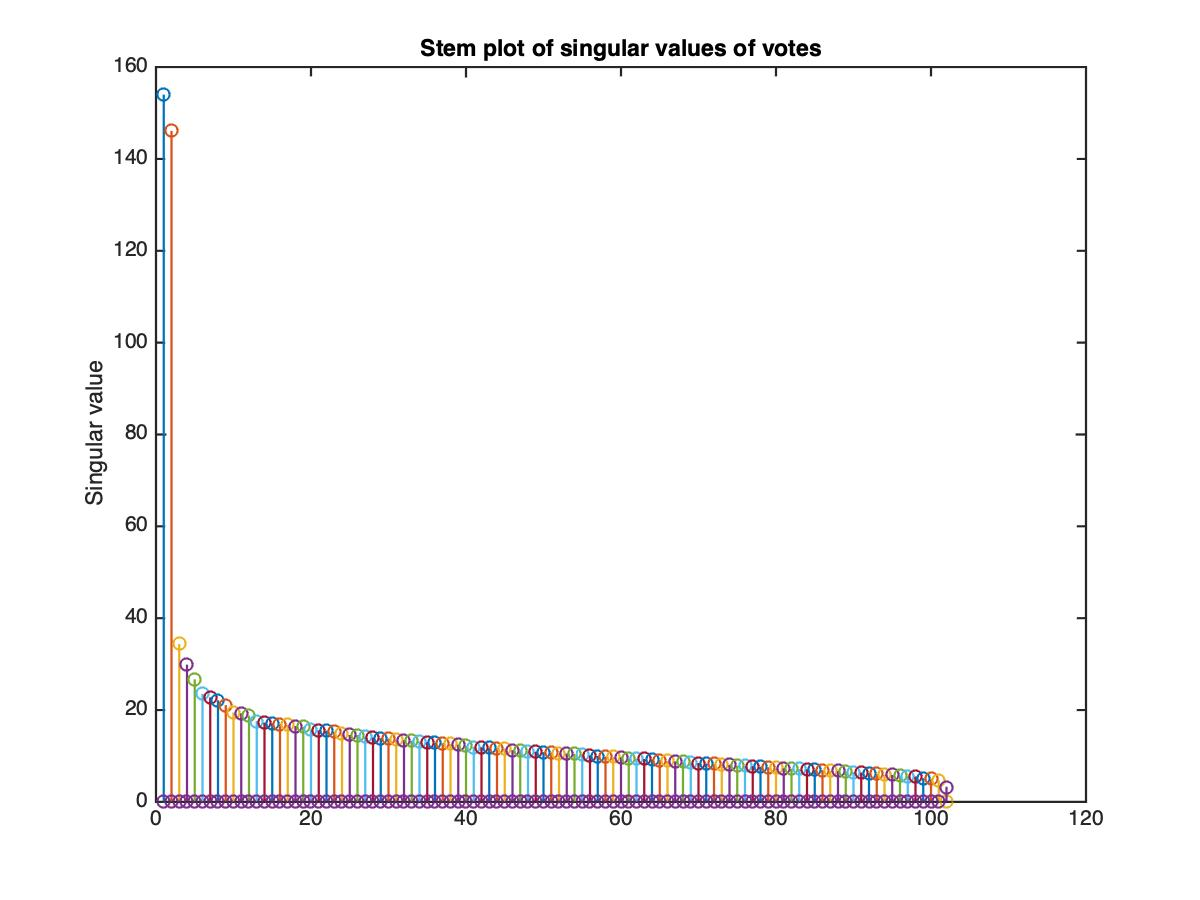
\includegraphics[scale=0.3]{final_data/stem_plot.jpg}
    \caption{Stem plot of singular values for votes matrix}
    \label{fig:step_plot}
  \end{figure}

  \begin{figure}[hpb!]
    \centering
    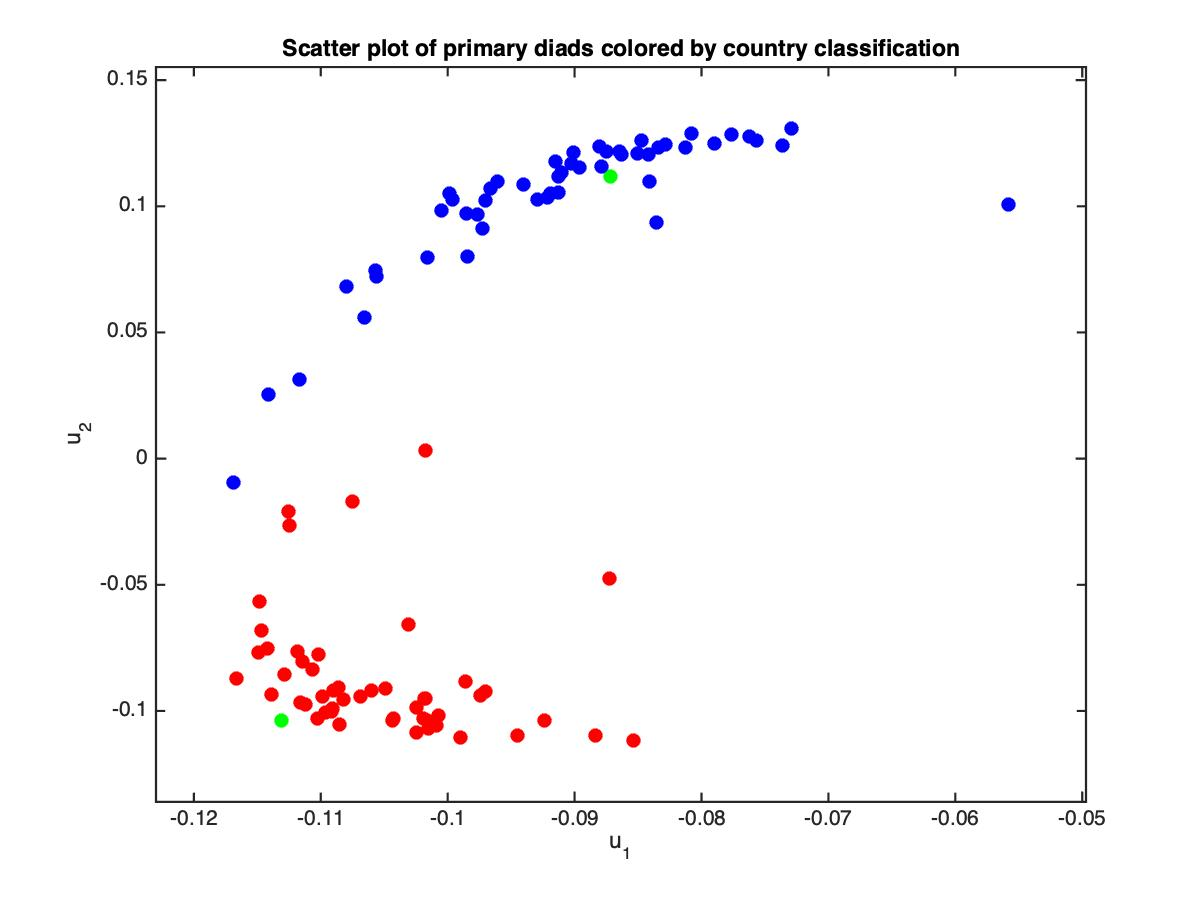
\includegraphics[scale=0.3]{final_data/country_scatter_classification.jpg}
    \caption{Scatter plot of $u_1$ and $u_2$ by country classification where Capitalists, Communists and Socialists are represented by red, blue, and green markers, respectively.}
    \label{fig:scatter_plot_by_country}
  \end{figure}

  \begin{figure}[hpb!]
    \centering
    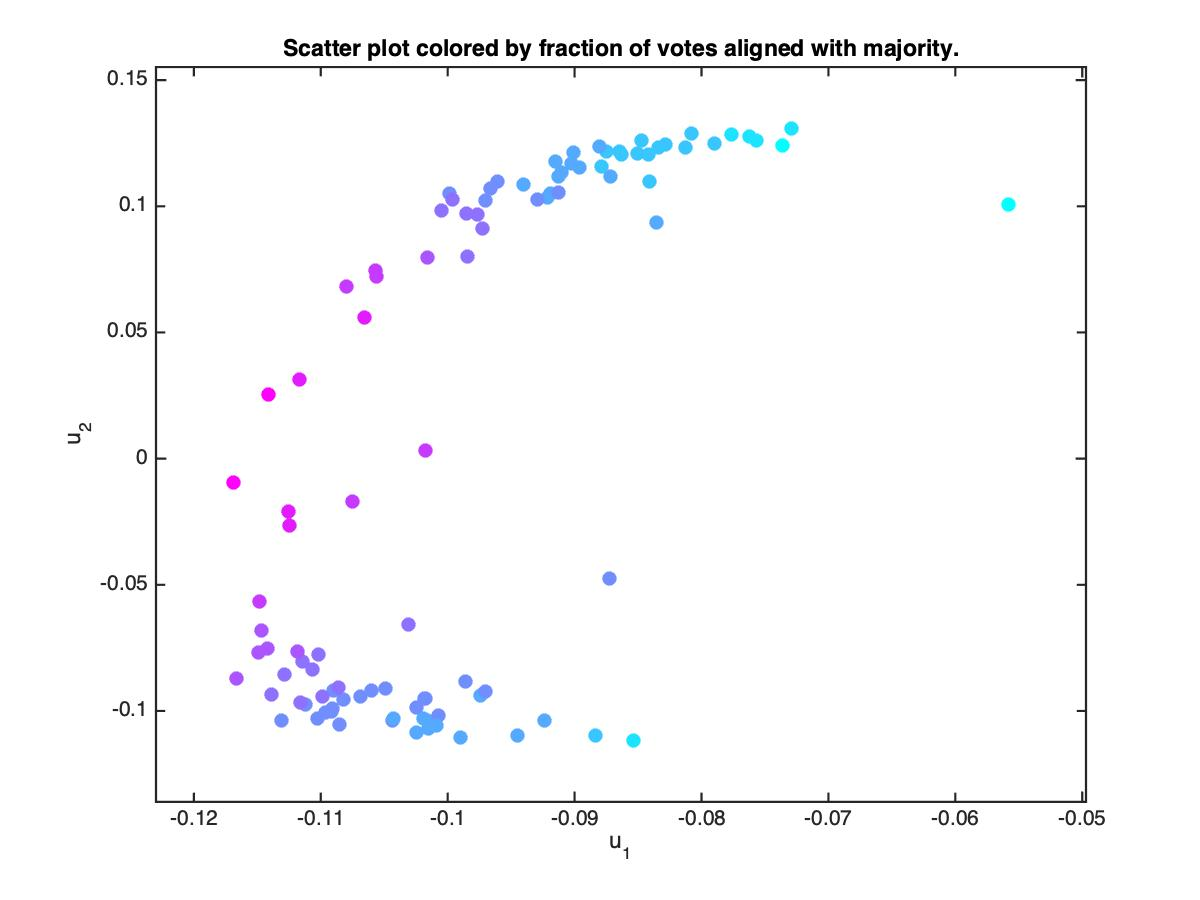
\includegraphics[scale=0.3]{final_data/country_majority_scatter_plot.jpg}
    \caption{Scatter plot of $u_1$ and $u_2$ showing the fraction of votes in which each country voted with the majority of the other countries. Pink implies large values, and blue small values.}
    \label{fig:scatter_plot_country_majority}
  \end{figure}

  \begin{figure}[hpb!]
    \centering
    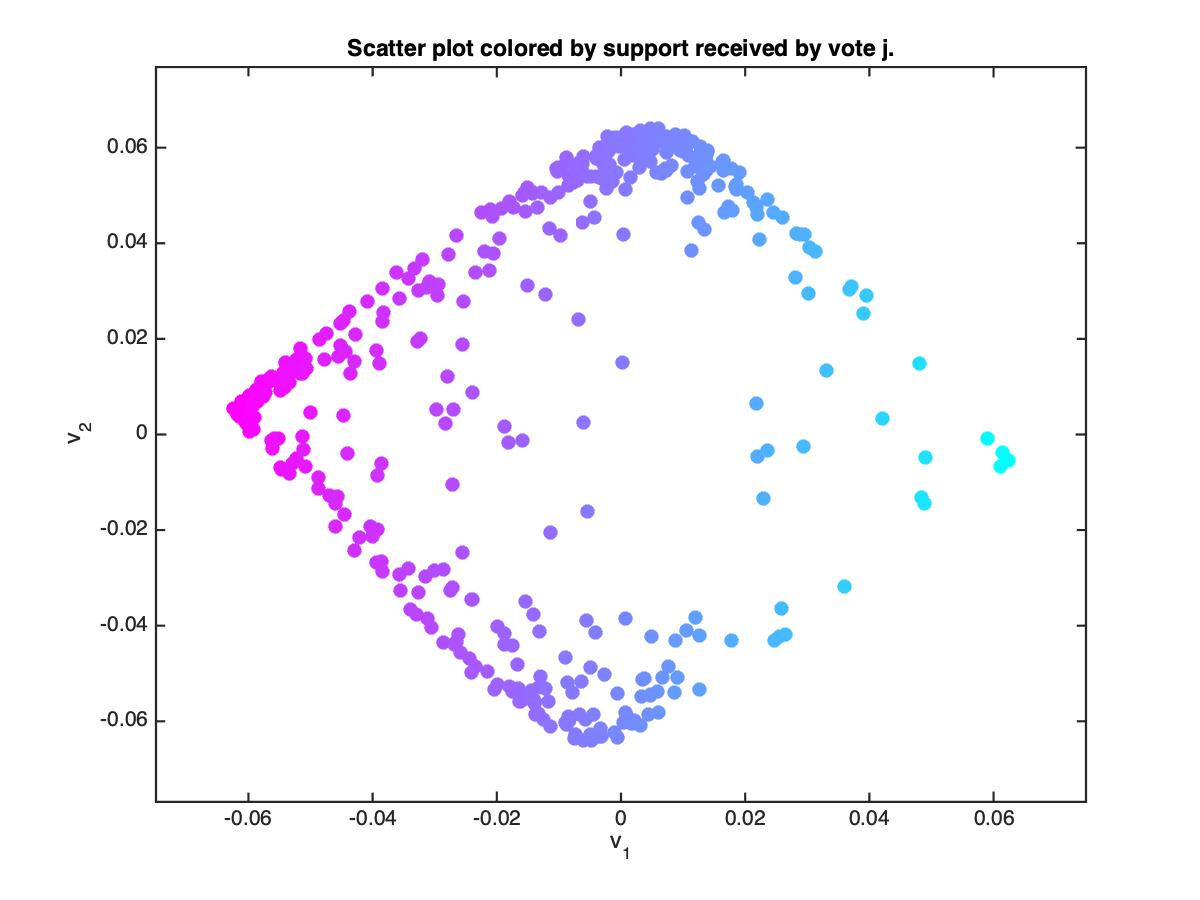
\includegraphics[scale=0.3]{final_data/votes_by_total_support.jpg}
    \caption{Scatter plot of $v_1$ and $v_2$ where colors indicate the total support received by vote $j$}
    \label{fig:scatter_plot_votes_by_total_support}
  \end{figure}

  \begin{figure}[hpb!]
    \centering
    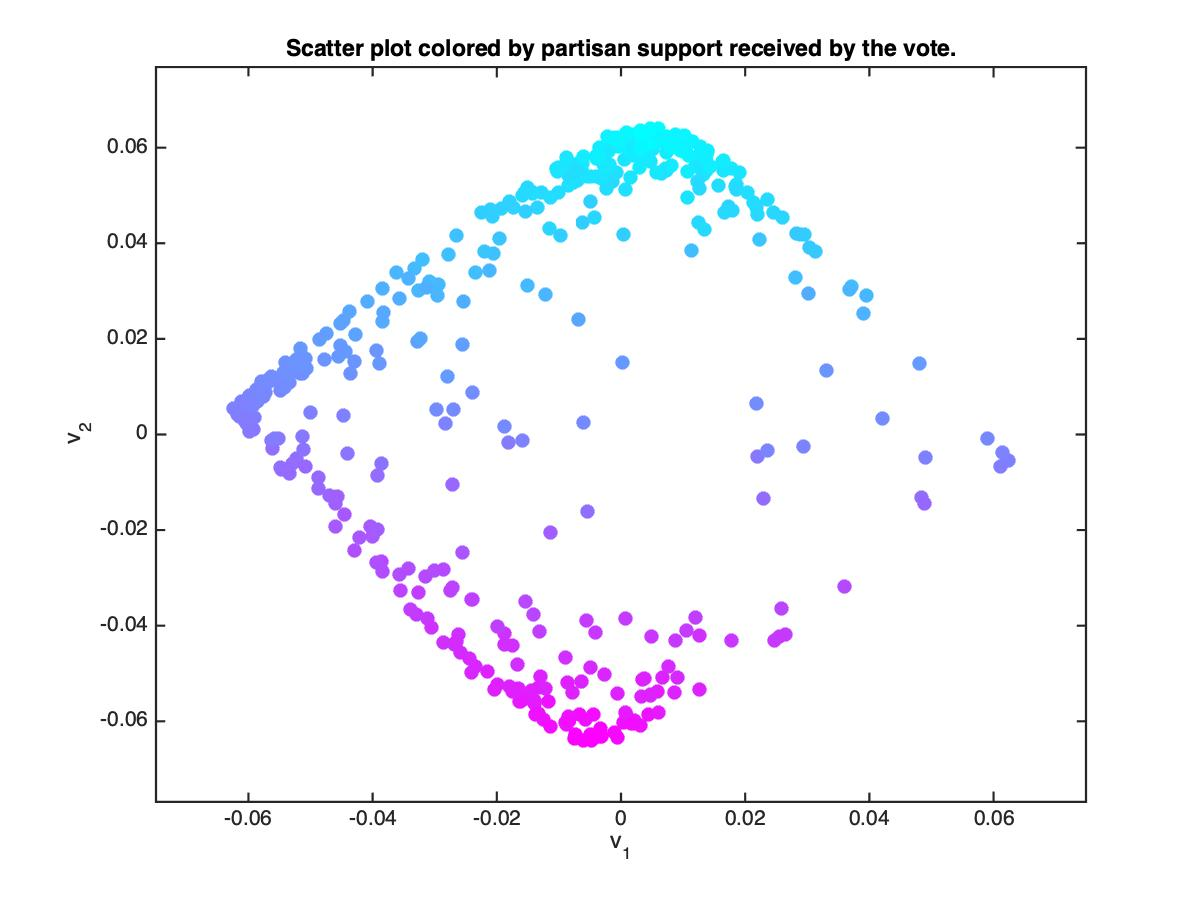
\includegraphics[scale=0.3]{final_data/votes_by_partisan_support.jpg}
    \caption{Scatter plot of $v_1$ and $v_2$ where the colors indicate the partisan support received by vote $j$}
    \label{fig:scatter_plot_votes_by_partisan_support}
  \end{figure}

\end{questions}

\includepdf[
    %% Include all pages of the PDF
    pages=-,
    %% make this page have the usual page style
    %% (you can change it to plain etc). By default pdfpages
    %% sets the pagecommand to \pagestyle{empty}
    pagecommand={\pagestyle{headings}}]
%% The pdf file itself
{FinalCode.pdf}















\end{document}
